Consider the following two functions.
%
\begin{figure}[h!]
  \center
  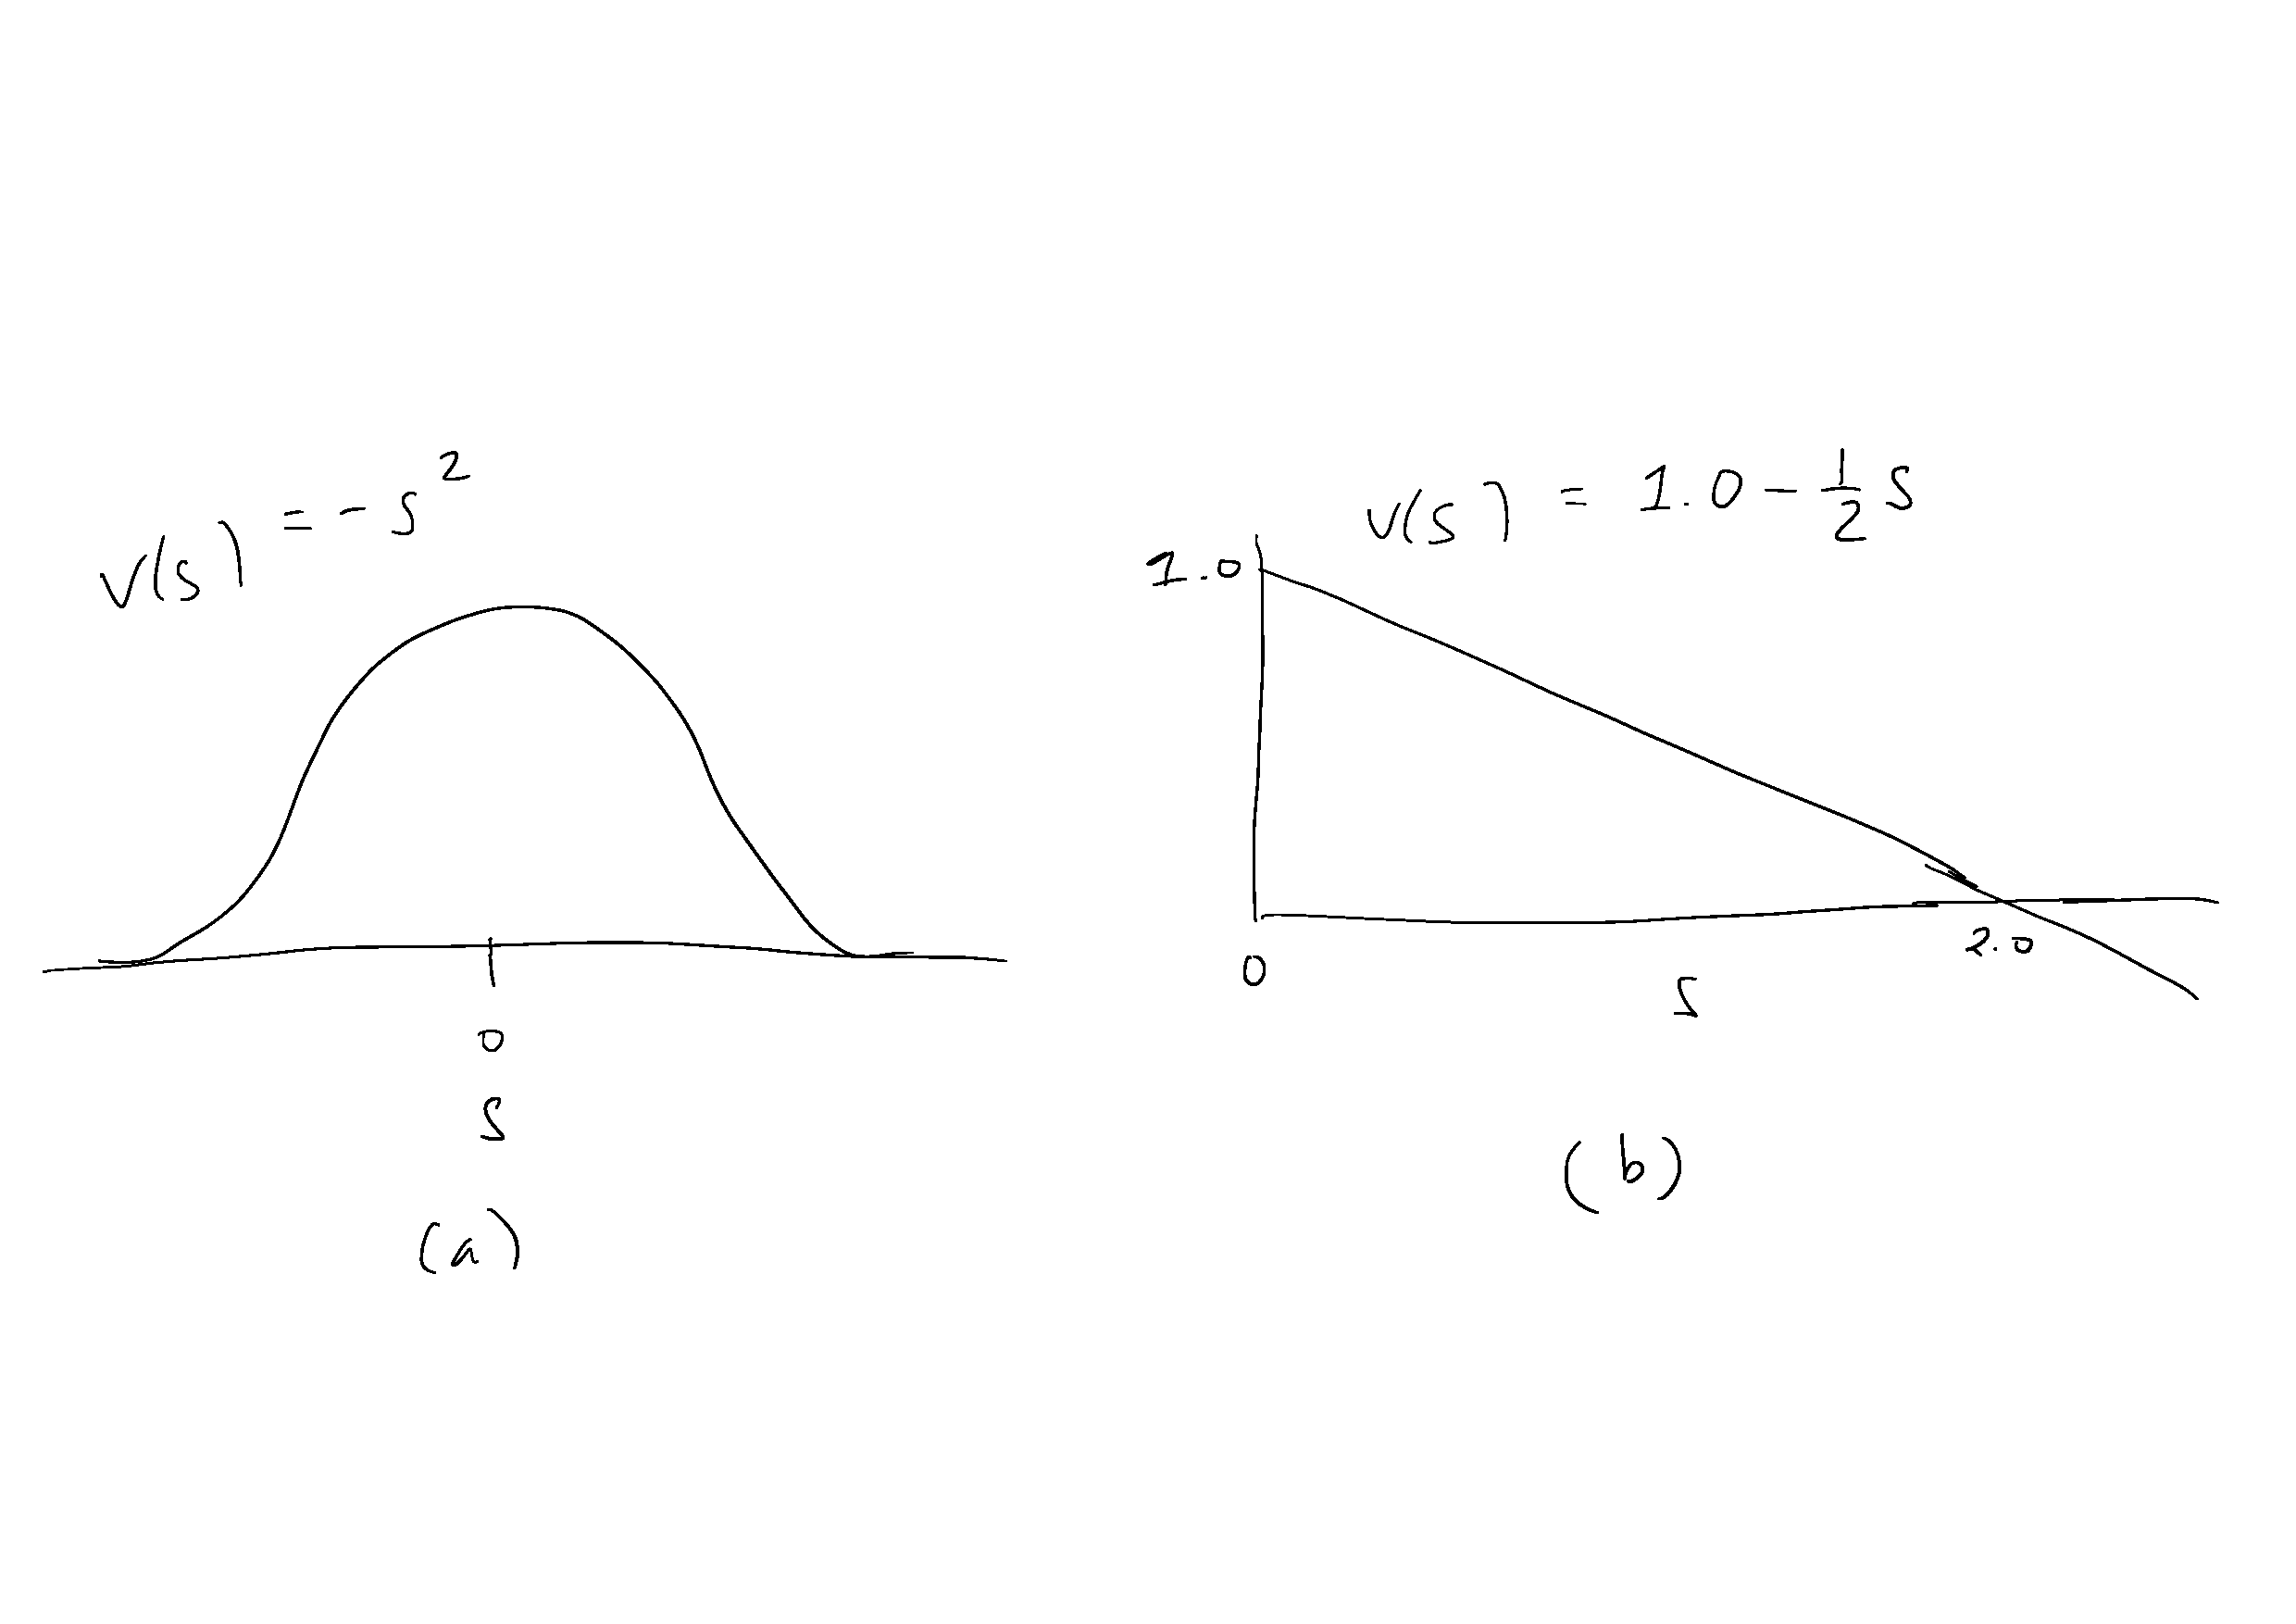
\includegraphics[width=0.75\linewidth]{figures/simplefcns.pdf}
\end{figure}
%
\begin{enumerate}
\item Design features for each function, to approximate them as a linear function of these features. Can you design features to make the approximation exact?
\item Can you design one set of features, that allows you to represent both functions?
\end{enumerate}
